\section{System's Perspective} \label{sec:system}
This section documents the architecture of the MiniTwit application. First, the individual dependencies of the application are presented and the rationale behind them. Next, we describe the current state of the system.

\subsection{Architecture \& Design}
The MiniTwit application relies on several dependencies, each interacting with each other in many ways. Figure \ref{fig:architecture} provides an overview of these interactions. In figure \ref{fig:architecture}, it can be seen that a pipeline of actions is initiated every time a commit is pushed to the MiniTwit GitHub repository. When a commit is pushed, the GitHub Actions initializes our CI/CD setup, which is described later in section \ref{sec:cicd}. This setup deploys the image of the application and all its dependencies, which are described in section \ref{sec:dependencies}, to the Docker Hub. From the Docker Hub, everything is deployed to DigitalOcean which hosts our application. On DigitalOcean we use a replication setup, described in section \ref{sec:scaling}, which ensures availability of the application.

\begin{figure}[H]
    \centering
    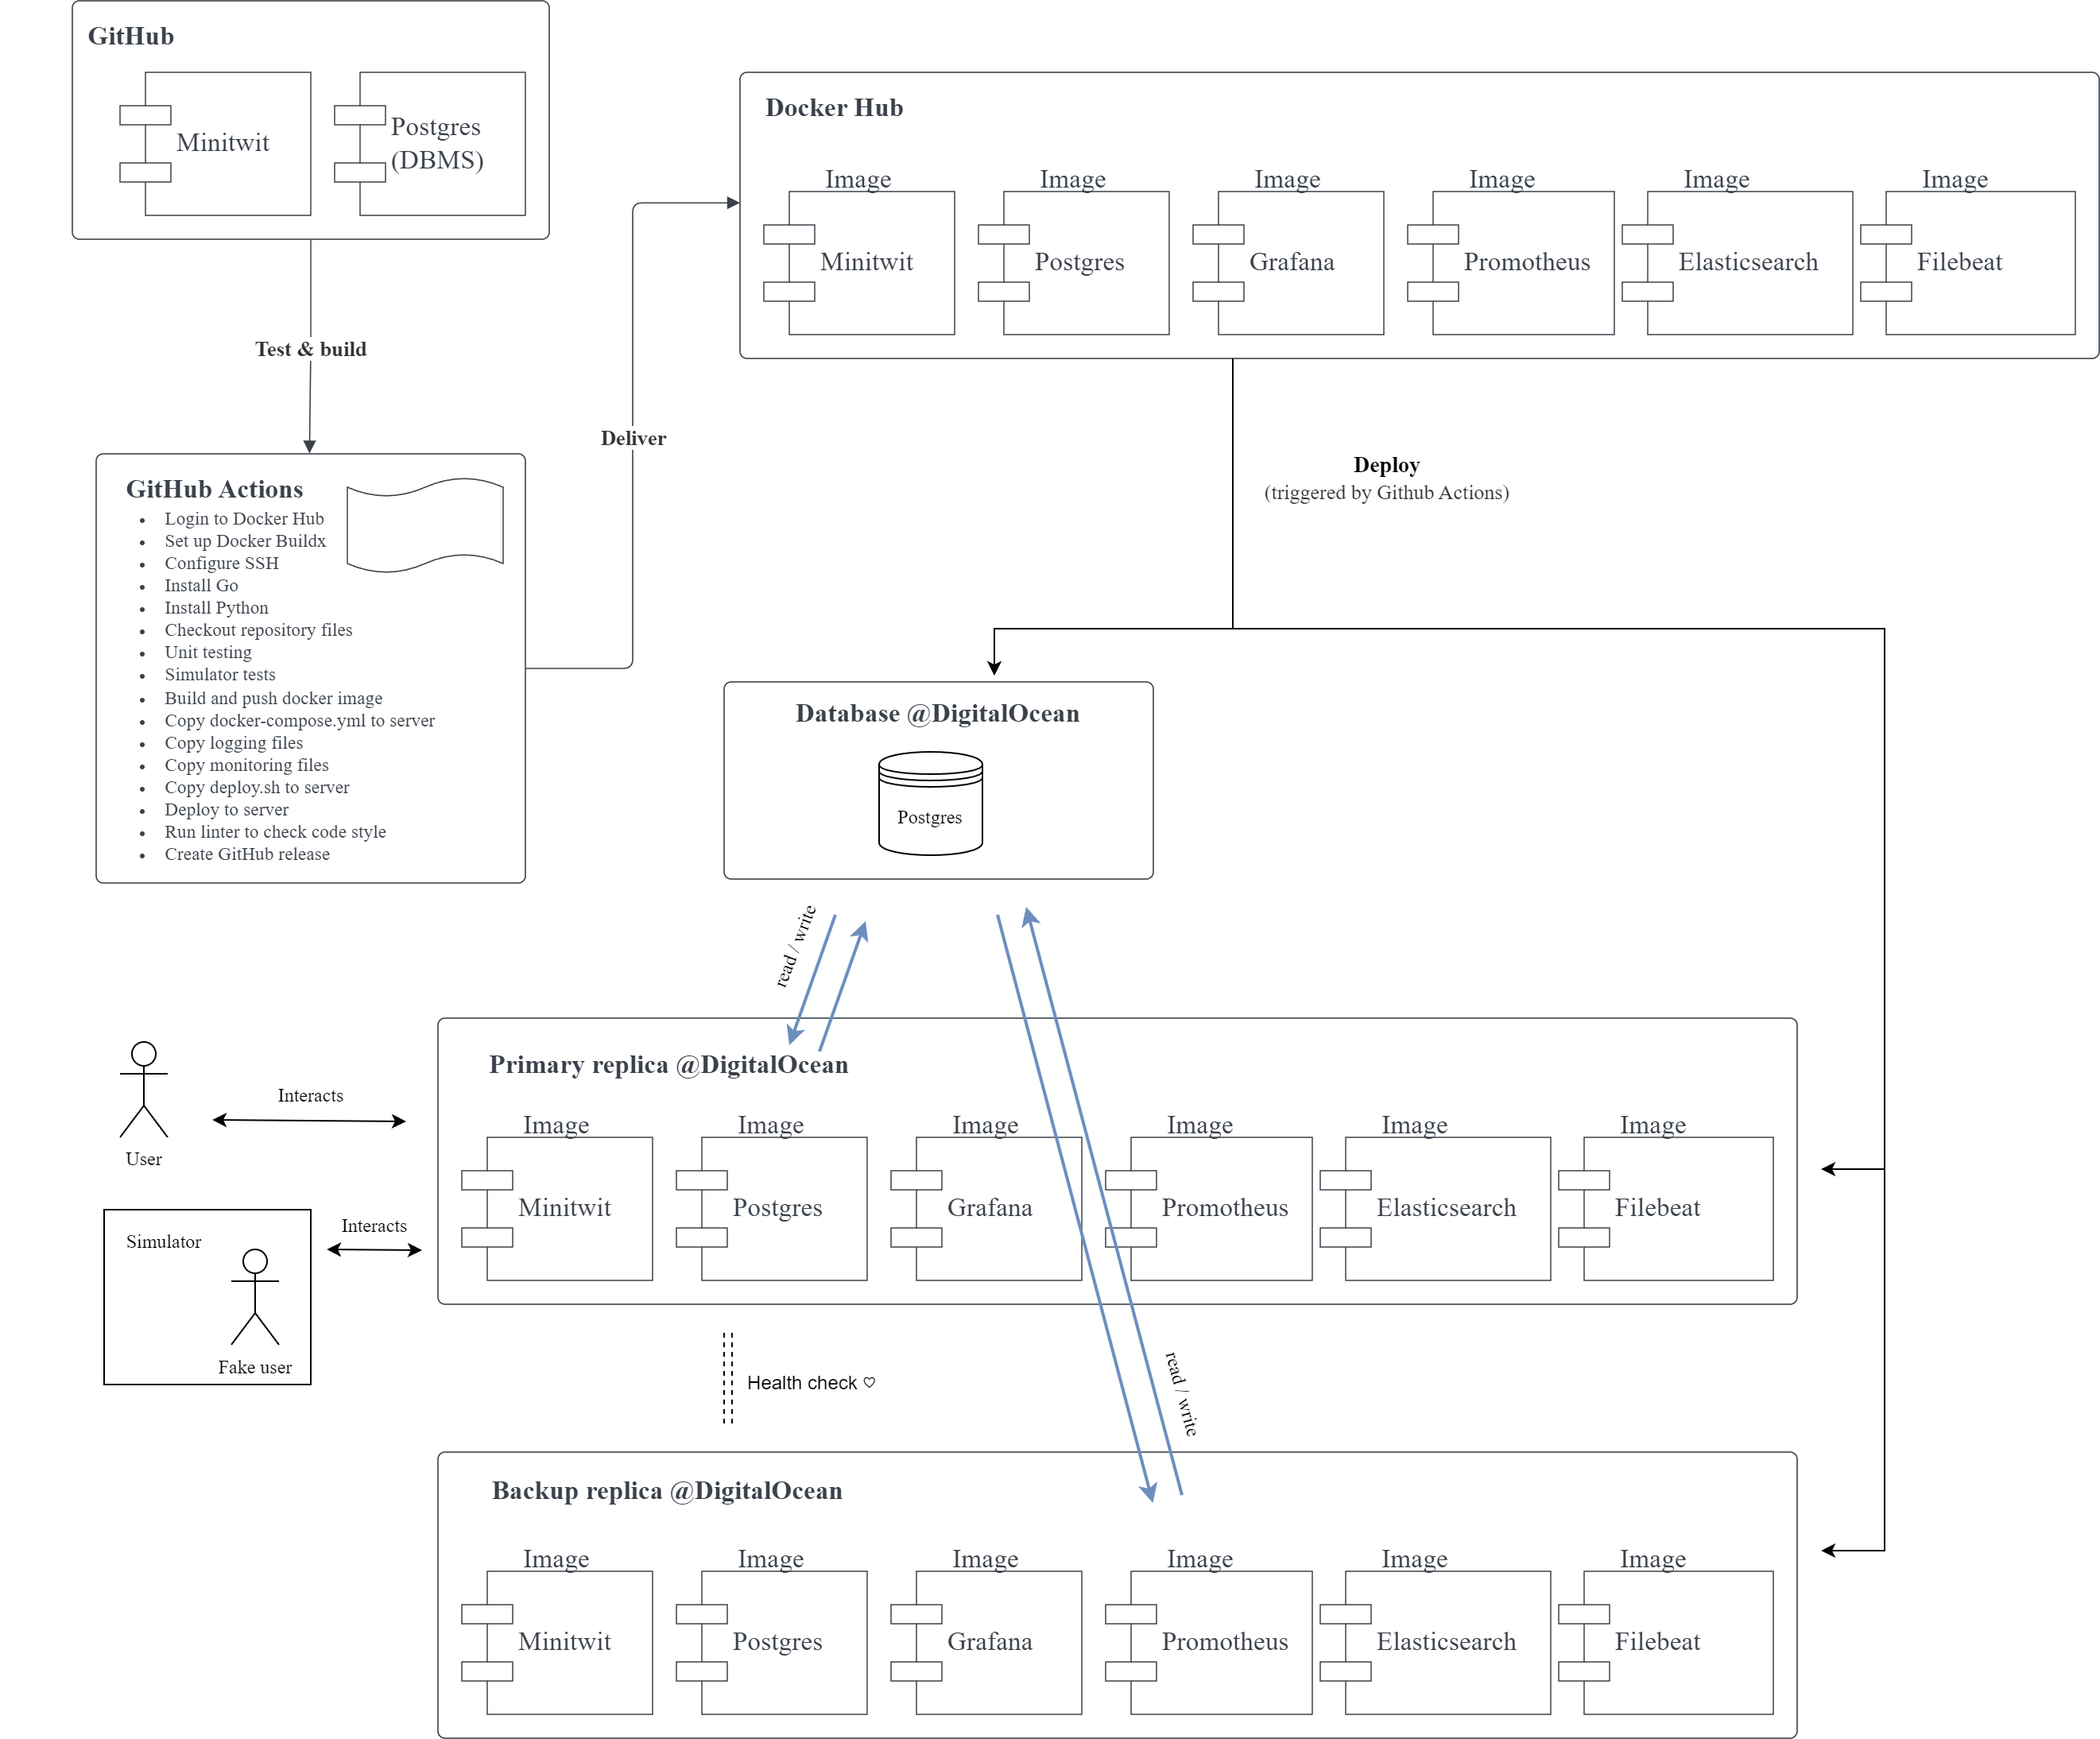
\includegraphics[width=\linewidth]{images/architecture.png}
    \caption{Architecture of the MiniTwit application. The diagram shows which dependencies are involved in the application, and how they interact with each other.}
    \label{fig:architecture}
\end{figure}

\subsection{Dependencies} \label{sec:dependencies}
%arguments for choice of technologies
This section describes the different dependencies used in our application, and we argue for the choice of each technology.

\paragraph*{Docker}
We utilize Docker\footnote{\href{https://www.docker.com/}{docker.com}} to containerize all our dependencies, making it easier to isolate and deploy our application. Without containerization, managing the various tools and their dependencies would be difficult, requiring multiple steps for each application run. Docker simplifies this process by packaging everything together and enabling us to execute the application with a single command. We chose Docker over alternatives like Kubernetes due to our prior experience with it and its ability to fulfill all our application requirements.

\paragraph*{Go \& Gin}
For our web-application, we opted to use Gin\footnote{\href{https://gin-gonic.com/}{gin-gonic.com}} as our web framework. Gin is a fast and stable web framework written for Go/Golang. We selected Gin due to its superior performance compared to other frameworks, including Flask, which was the original framework used in the MiniTwit application. We specifically required a web framework that supports HTML rendering and relational databases, as we wanted to be maximize reuse of the original MiniTwit application. Gin fulfills these requirements while also offering scalability and type safety, which are useful for writing maintainable code. Moreover, this project provided us with an ideal opportunity to learn Go and utilize Gin.

\paragraph*{Gorm}
In Go programming, one of the most popular ORM (Object–relational mapping) libraries is Gorm\footnote{\href{https://gorm.io/}{gorm.io}}. Our decision to employ Gorm was driven by its maturity and reputation within the Go community. Gorm encompasses all the essential ORM functionalities we required, such as database object creation, retrieval, updating, and deletion. With Gorm, we were able to effortlessly define Go objects with the necessary fields for smooth integration with our database.

\paragraph*{Vagrant}
In our project, we employ Vagrant\footnote{\href{https://www.vagrantup.com/}{vagrantup.com}} to streamline the configuration and deployment of the virtual machine that hosts our application on the DigitalOcean server. Vagrant allows us to give an generic description of the virtual machine we need, which it utilizes to create the virtual machine. This eliminates the need for manual interaction with programs like VirtualBox, sparing us from navigating through UIs. By automating this process, we mitigate the risk of errors during each VM setup, ensuring consistency in our deployments. Vagrant was selected over alternative solutions due to its versatility and compatibility with various containerization platforms, seamlessly integrating with different development ecosystems. Furthermore, it provides cross-platform support for Windows, MacOS, and Linux, making it a suitable choice for our diverse operating system requirements.

\paragraph*{Prometheus \& Grafana}
We have adopted Prometheus\footnote{\href{https://prometheus.io/}{prometheus.io}} to extract valuable insights from our Minitwit application due to the following reasons: Prometheus offers extensive support for a wide range of metrics, making it highly versatile for monitoring needs. It seamlessly integrates with the Go programming language. By utilizing Prometheus, we can effortlessly integrate it with popular dashboard tools like Grafana\footnote{\href{https://grafana.com/}{grafana.com}}, enabling us to create visually appealing and informative dashboards. In addition, Prometheus allows us to set up alerts that notify our team whenever certain metrics exceed predefined thresholds. In conjunction with Prometheus, we utilize Grafana to visualize the data collected. We specifically chose Grafana for its user-friendly interface and ability to create highly customizable dashboards that require minimal configuration efforts.

\paragraph*{Elasticsearch, Filebeat \& Kibana}
To facilitate logging in our Minitwit application, we implemented the EFK stack. This stack proves to be an ideal solution for our needs, offering several key advantages. Firstly, it incorporates Filebeat, a lightweight log shipper that collects, parses, and forwards logs from our application to a storage component. This log transportation ensures efficient and reliable log management. Secondly, the stack utilizes Elasticsearch as an efficient storage and analytics engine, enabling us to handle large volumes of data while providing excellent full-text search capabilities. Lastly, Kibana, the dashboard component of the EFK stack, simplifies setup and offers a user-friendly interface for filtering queries on the data stored in Elasticsearch. With Kibana, we can easily access and display the most valuable log data based on our requirements. 

\paragraph*{DigitalOcean}
Our chosen cloud infrastructure provider is DigitalOcean\footnote{\href{https://www.digitalocean.com/}{digitalocean.com}}. DigitalOcean stands ouut for its user-friendly interface, specifically designed for setting up and deploying Droplets (VMs) and Volumes (storage). In general, the platform is known for its simplicity and affordability, which aligns perfectly with the requirements for our Minitwit application. DigitalOcean's reputation for simplicity and affordability, combined with a student benefit they offer, makes it an ideal choice for our Minitwit application. It allows us to effectively manage our infrastructure within our budget while taking advantage of the student benefit.

\paragraph*{GitHub \& GH Actions}
To streamline our CI/CD workflow, we utilize GitHub Actions due to it being integrated in GitHub, which is our chosen version control system. By utilizing GitHub Actions, we consolidate our workflow within a single platform, eliminating the need for multiple tools. Additionally, it being integrated in GitHub allows us to conveniently track the status of individual commits as we push them. This visibility enables us to promptly identify build errors or failures in tests associated with specific commits. Furthermore, GitHub Actions allows for Continuous Delivery and Deployment capabilities, automating the process of delivering and deploying changes seamlessly using the same system.

\subsection{Current state of the system}
At the time of writing (20-05-2023) our static code analysis tools, which are explained in section \ref{sec:cicd}, report the following:
\begin{itemize}
    \item \textbf{Sonarcloud}: Latest pull request passed with 0 bugs, 0 vulnerabilities, 0 security hotspots and 10 code smells. We have assessed the code smells and decided to ignore them as they are insignificant.
    \item \textbf{Snyk}: It is currently disabled as it caused issues that blocked our CI/CD chain. We have not prioritized to fix the underlying problem as we believe the other code analysis tools provide a satisfying coverage of potential security vulnerabilities.
    \item \textbf{CodeQL}: Latest deployment passed CodeQL in the CI/CD chain.
    \item \textbf{Dependabot}: No active pull requests for vulnerable dependencies.
    \item \textbf{Lint for Go}: Latest deployment passed Lint in the CI/CD chain.
\end{itemize}

\subsection{License compatibility}
Our project is under GPL 3.0 which is compatible\footnote{\href{https://www.gnu.org/licenses/license-list.en.html}{gnu.org/licenses/license-list.en.html}} with all dependencies, namely: \textit{MIT License}, \textit{GNU Affero General Public License v3.0}, \textit{Apache License 2.0}, \textit{Server Side Public License}, \textit{ISC}, \textit{BSD-3-Clause}. 

